\chapter{Modelagem Físico Matemática}\label{cap:ferramentas}

\section{Sistemas de Coordenadas e Sistema de Medida de Tempo}\label{sec:3.1.1}

É de fundamental importância para qualquer estudo da mecânica a determinação objetiva dos sistemas de referência, sendo eles o de coordenadas e o de tempo. O parâmetro para essa escolha é a facilitação da formulação, visualização e análise dos fenômenos e resultados.

\subsection{Sistema de Coordenadas Geocêntrico-Equatorial Inercial (SCGI)}\label{sec:3.1.1.1}

Por conta do tempo do fenômeno ser insignificante em relação à variação das direções e origem do sistema de coordenadas, é assumido como hipótese simplificadora que esse sistema é não rotacional e fixo no espaço, \textit{i.e.}, inercial. 

O sistema de coordenadas geocêntrico-equatorial inercial \begin{math}I\end{math} tem como origem o centro de massa da Terra, \textit{i.e.}, geocêntrico, e base composta pelos vetores \begin{math}\{\vec{i}_1,\vec{i}_2,\vec{i}_3\}\end{math}. O eixo $\vec{i}_1$ tem como sentido o equinócio vernal $\Upsilon$, o eixo $\vec{i}_3$ aponta para a normal do plano (fundamental) equatorial terrestre, \textit{i.e.}, o polo Norte celeste e o eixo $\vec{i}_2$ completa a base ortogonal dextrogiro \cite[p.~12-13]{zanardi2018}. Mostrado na Figura~\ref{fig:11}.

\begin{figure}[htpb]
\centering
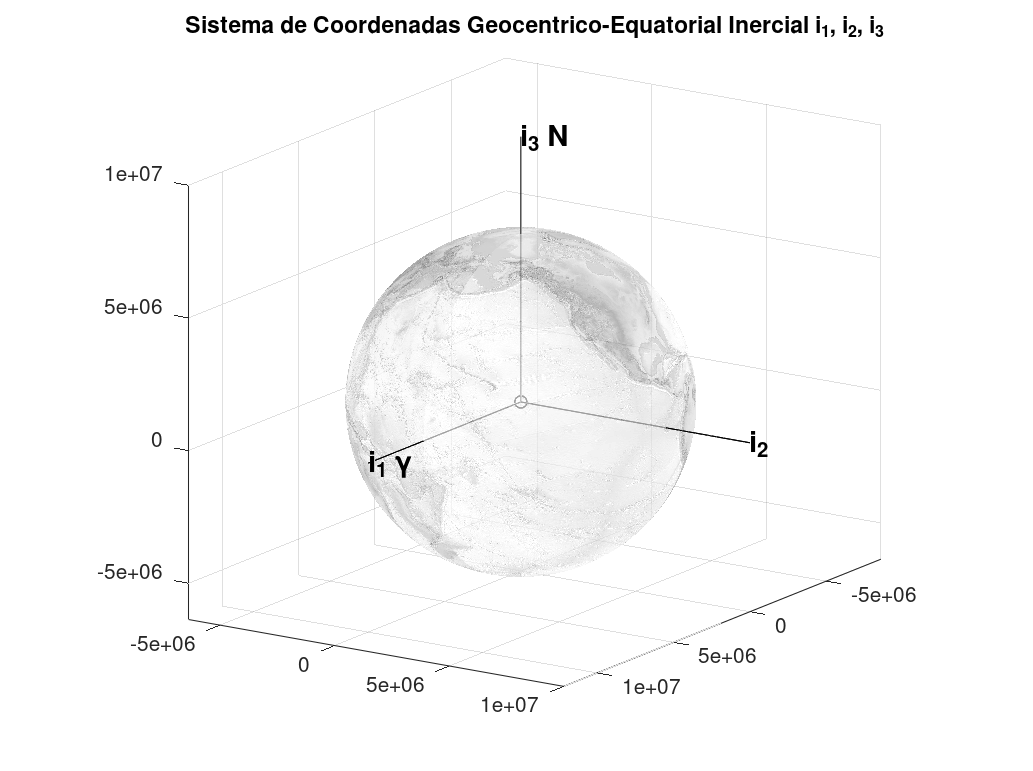
\includegraphics[scale=0.3]{figs/SCGI.png}
\caption{Sistema de Coordenada Geocêntrico-Equatorial Inercial (SCGI)}
\label{fig:11}
\end{figure}

\subsection{Sistema de Coordenadas Orbital (SCO)}\label{sec:3.1.1.2}

O sistema de coordenadas orbital \begin{math}O\end{math} tem como origem o centro de massa do veículo espacial em órbita e base composta pelos vetores \begin{math}\{\vec{o}_1,\vec{o}_2,\vec{o}_3\}\end{math}. O eixo $\vec{o}_3$ aponta em direção ao centro de massa da Terra ou, direção nominal do nadir. O eixo $\vec{o}_2$ tem como direção o oposto do vetor do plano fundamental de órbita do veiculo espacial \cite[p.~26-29]{wertz2012spacecraft}. E o eixo $\vec{o}_1$ aponta para o vetor velocidade nominal ou, a direção nominal da trajetória da órbita. Representado na Figura~\ref{fig:12}.

\begin{figure}[htpb]
\centering
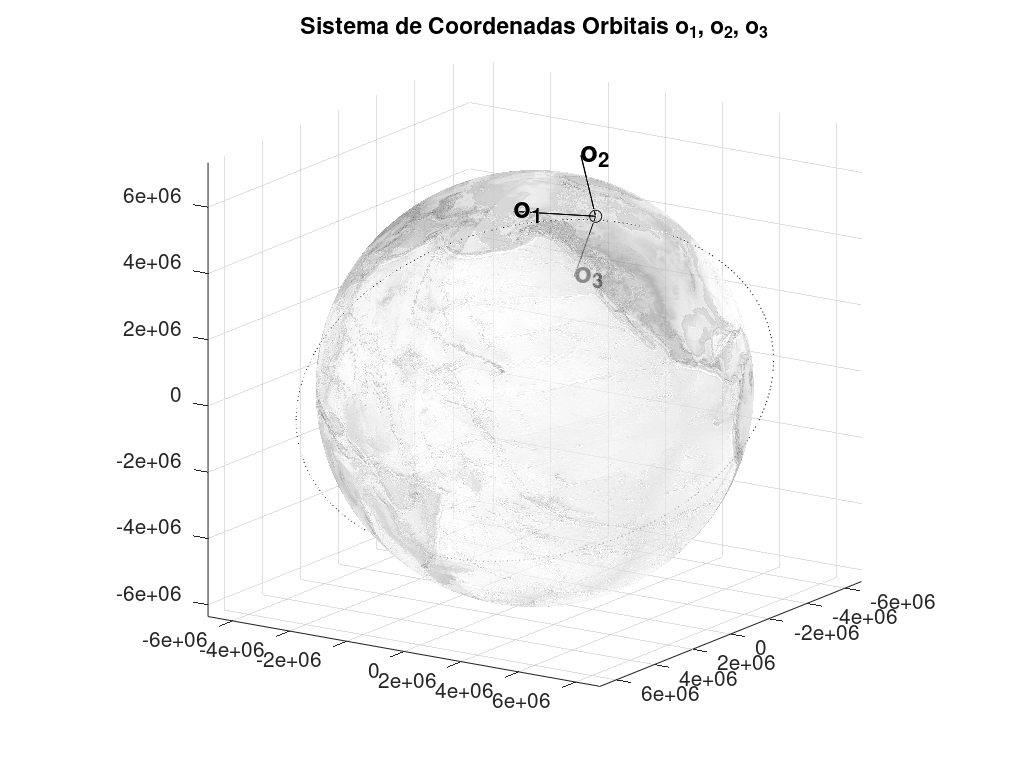
\includegraphics[scale=0.3]{figs/SCO.png}
\caption{Sistema de Coordenada Orbital (SCO)}
\label{fig:12}
\end{figure}

\subsection{Sistema de Coordenadas Fixo no Corpo (SCFC)}\label{sec:3.1.1.3}

O sistema de coordenadas fixo no corpo, \begin{math}B\end{math}, tem como origem o centro de massa do veículo espacial, sua base é composta pelos vetores \begin{math}\{\vec{b}_1,\vec{b}_2,\vec{b}_3\}\end{math}, sendo escolhidos arbitrariamente. É interessante alinhar esses eixos com as direções dos eixos principais de inércia. Escolhendo eixo $\vec{b}_3$ como eixo de Spin, \textit{i.e.}, o eixo de menor momento principal de inércia. Os eixos $\vec{b}_2$, $\vec{b}_1$ o segundo e o terceiro menores momentos principais de inércia \cite[p.~26-29]{wertz2012spacecraft}. Como representado na Figura~\ref{fig:13}.

\begin{figure}[htpb]
\centering
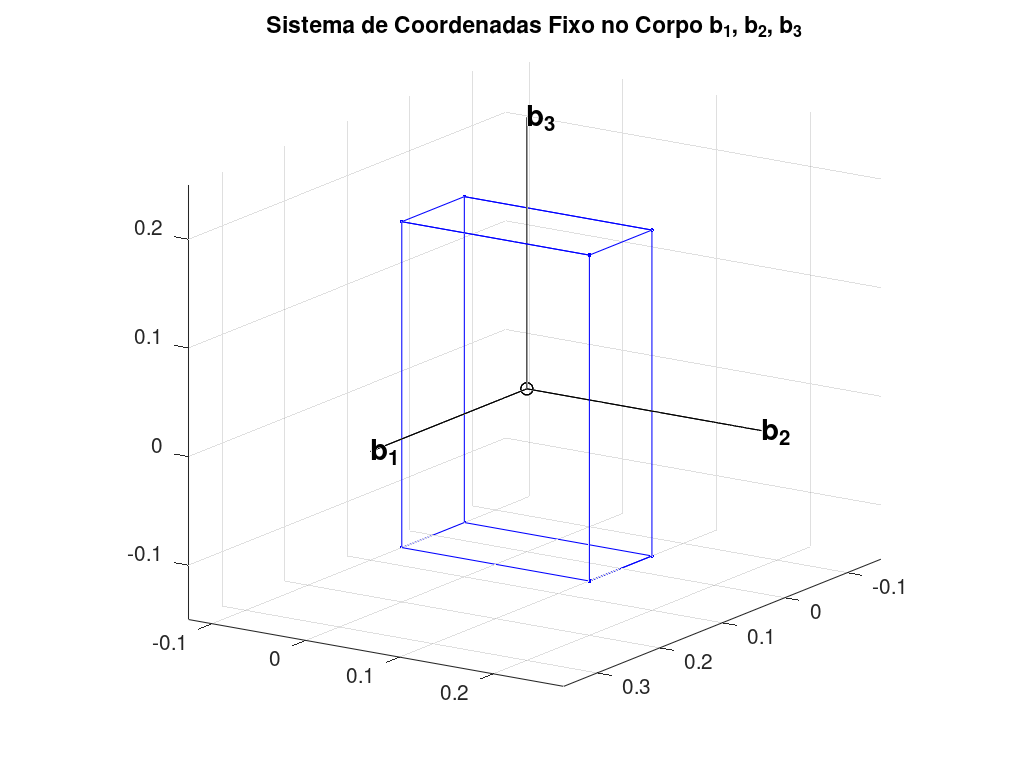
\includegraphics[scale=0.3]{figs/SCBF.png}
\caption{Sistema de Coordenada Fixo no Corpo (SCFC)}
\label{fig:13}
\end{figure}

\subsection{Sistema de Referência de Tempo}\label{sec:3.1.1.4}

A referência para os sistemas de coordenadas descritos acima é o equador médio e o equinócio vernal referente a data Gregoriana de 1º de Janeiro de 2000 às 12 horas U.T. (tempo universal) ou a data Juliana de 2451545. Esse sistema de referência é conhecido como J2000. É a escolha dessa referência que garante que o sistema de coordenadas Geocêntrico-equatorial possa ser considerado não rotacional \cite{schutz2004statistical}.

\section{Mecânica Rotacional}\label{sec:3.1.2}

Nesta seção estuda-se a representação da cinemática rotacional de um corpo rígido. Entende-se que essa formulação é a mesma usada em um modelo de CubeSat. Sendo o principal objetivo descrever a orientação e rotação do corpo.

Existem várias maneiras de representar a atitude de um corpo rígido e a depender do propósito, visualização ou cálculo, umas são mais indicadas que outras. Temos entre elas a matriz de cossenos diretores, os ângulos de Euler, o Eixo-ângulo de Euler e os parâmetros de Euler (Quatérnions).

A formulações a seguir seguem a literatura \cite[p.~323-486]{wie2008space}

\subsection{Matriz de Cossenos Diretores}\label{sec:3.1.2.1}

Considerando o sistema \begin{math}A\end{math} e \begin{math}B\end{math} como dextrogiros e compostos por três vetores unitários ortonormais (versores) cada, sendo respectivamente \begin{math}A = \{\vec{a_1}, \vec{a_2}, \vec{a_3}\}\end{math} e \begin{math}B = \{\vec{b_1}, \vec{b_2}, \vec{b_3}\}\end{math}.

Pode-se expressar  os versores da base \begin{math}B\end{math} em termos da base \begin{math}A\end{math} como mostrado abaixo:

\begin{equation}
\begin{bmatrix}
\vec{b_1} \\ \vec{b_2} \\ \vec{b_3}
\end{bmatrix}
=
\begin{bmatrix}
C_{11} & C_{12} & C_{13} \\ C_{21} & C_{22} & C_{23} \\ C_{31} & C_{32} & C_{33}
\end{bmatrix}
\begin{bmatrix}
\vec{a_1} \\ \vec{a_2} \\ \vec{a_3}
\end{bmatrix}
=
C^{B/A}
\begin{bmatrix}
\vec{a_1} \\ \vec{a_2} \\ \vec{a_3}
\end{bmatrix} \;
\end{equation}

\begin{math}C^{B/A}\end{math} é conhecido como a matriz de cossenos diretores. Descreve a orientação de \begin{math}B\end{math} em relação a \begin{math}A\end{math}.

Podendo ser escrita da forma a seguir:

\begin{equation}
C^{B/A}
=\begin{bmatrix}
\vec{b_1}\cdot \vec{a_1} & \vec{b_1}\cdot \vec{a_2} & \vec{b_1}\cdot \vec{a_3} \\ \vec{b_2}\cdot \vec{a_1} & \vec{b_2}\cdot \vec{a_2} & \vec{b_2}\cdot \vec{a_3} \\ \vec{b_3}\cdot \vec{a_1} & \vec{b_3}\cdot \vec{a_2} & \vec{b_3}\cdot \vec{a_3}
\end{bmatrix}=
\begin{bmatrix}
\vec{b_1} \\ \vec{b_2} \\ \vec{b_3}
\end{bmatrix}
\cdot
\begin{bmatrix}
\vec{a_1} & \vec{a_2} & \vec{a_3}
\end{bmatrix}
\end{equation}

A matriz de cossenos diretores é conhecida como: matriz de rotação ou matriz de transformação de coordenadas de \begin{math}A\end{math} para \begin{math}B\end{math}. Tal transformação de coordenada é representada simbolicamente como \begin{math}C^{B/A}:B\leftarrow A\end{math}

Por simplicidade, muitas vezes representa-se essa matriz simplesmente por \begin{math}C\end{math}. Algumas propriedades da matriz \begin{math}C\end{math} são:

\begin{equation}C^{-1}=C^T\end{equation}

Que é equivalente a:

\begin{equation}CC^T=I=C^TC\end{equation}

Isso ocorre pois C é uma matriz ortogonal. Consequentemente tem-se as seguinte relações entre \begin{math}C^{A/B}\end{math} e \begin{math}C^{B/A}\end{math}: 

\begin{equation}
\left[C^{A/B}\right]_{ij}=\vec{a}_i\cdot\vec{b}_j
\end{equation}
\begin{equation}
\left[C^{B/A}\right]_{ij}=\vec{b}_i\cdot\vec{a}_j
\end{equation}
\begin{equation}
\left[C^{A/B}\right]^{-1}=\left[C^{A/B}\right]^T=C^{B/A}
\end{equation}
\begin{equation}
\left[C^{B/A}\right]^{-1}=\left[C^{B/A}\right]^T=C^{A/B}
\end{equation}

Assim dados dois conjuntos de sistema de coordenadas, \begin{math}A\end{math} e \begin{math}B\end{math}, e um vetor arbitrário \begin{math}\vec{H}\end{math}, esse pode ser expresso em termos dos vetores da base A e B:

\begin{equation}
\vec{H}=H_1\vec{a_1}+H_2\vec{a_2}+H_3\vec{a_3}
\end{equation}
\begin{equation}
=H'_1\vec{b_1}+H'_2\vec{b_2}+H'_3\vec{b_3}
\end{equation}

De onde se adquire:

\begin{equation}
\begin{bmatrix}
H'_1 \\ H'_2 \\ H'_3
\end{bmatrix}
=
\begin{bmatrix}
\vec{b_1}\cdot \vec{a_1} & \vec{b_1}\cdot \vec{a_2} & \vec{b_1}\cdot \vec{a_3} \\ \vec{b_2}\cdot \vec{a_1} & \vec{b_2}\cdot \vec{a_2} & \vec{b_2}\cdot \vec{a_3} \\ \vec{b_3}\cdot \vec{a_1} & \vec{b_3}\cdot \vec{a_2} & \vec{b_3}\cdot \vec{a_3}
\end{bmatrix}
\begin{bmatrix}
H_1 \\ H_2 \\ H_3
\end{bmatrix}
=
C^{B/A}
\begin{bmatrix}
H_1 \\ H_2 \\ H_3
\end{bmatrix}
\end{equation}Três rotações elementares respectivamente: no primeiro, no segundo e no terceiro eixos, da referência \begin{math}A\end{math}, são descritas com as matrizes de rotação a seguir:

\begin{equation}C_1(\theta_1)=
\begin{bmatrix}
1 & 0 & 0 \\ 0 & cos\theta_1 & sen\theta_1 \\ 0 & -sen\theta_1 & cos\theta_1 
\end{bmatrix}
\end{equation}
\begin{equation}C_2(\theta_2)=
\begin{bmatrix}
cos\theta_2 & 0 & -sen\theta_2 \\ 0 & 1 & 0 \\ sen\theta_2 & 0 & cos\theta_2
\end{bmatrix}
\end{equation}
\begin{equation}
C_3(\theta_3)=
\begin{bmatrix}
cos\theta_3 & sen\theta_3 & 0 \\ -sen\theta_3 & cos\theta_3 & 0 \\ 0 & 0 & 1
\end{bmatrix}
\end{equation}

Onde \begin{math}C_i(\theta_i)\end{math} denota a direção da matriz de cossenos diretores \begin{math}C\end{math} para um rotação elementar sobre o eixo \begin{math}i\end{math} de \begin{math}A\end{math} com um ângulo de \begin{math} \theta_i \end{math}.

\subsection{Ângulos de Euler}\label{sec:3.1.2.2}

Existem 12 combinações para os ângulos de Euler. Elas são provindas performando rotações sucessivas sobre os eixos fixos de um corpo, onde cada rotação é efetuada em um eixo diferente daquele imediatamente anterior. Isso garante que é possível adquirir qualquer orientação arbitrária efetuando três rotações sucessivas sobre uma base fixa de referência.

Considere abaixo o exemplo da combinação de três rotações sucessivas nos eixos 321 fixo no corpo, que descrevem a orientação do sistema de referência \begin{math} B \end{math} em relação a referência \begin{math} A \end{math}.

Uma sequência particular é descrita abaixo:

\begin{equation}C_3(\theta_3): \; A'\leftarrow A\end{equation}
\begin{equation}C_2(\theta_2): \; A''\leftarrow A'\end{equation}
\begin{equation}C_1(\theta_1): \; B\leftarrow A''\end{equation}

E cada rotação pode ser descrita como:

\begin{equation}
\begin{bmatrix}
\vec{a'_1} \\ \vec{a'_2} \\ \vec{a'_3}
\end{bmatrix}
=
\begin{bmatrix}
cos\theta_3 & sen\theta_3 & 0 \\ -sen\theta_3 & cos\theta_3 & 0 \\ 0 & 0 & 1
\end{bmatrix}
\begin{bmatrix}
\vec{a_1} \\ \vec{a_2} \\ \vec{a_3}
\end{bmatrix}
=
C_3(\theta_3)
\begin{bmatrix}
\vec{a_1} \\ \vec{a_2} \\ \vec{a_3}
\end{bmatrix}
\end{equation}
\begin{equation}
\begin{bmatrix}
\vec{a''_1} \\ \vec{a''_2} \\ \vec{a''_3}
\end{bmatrix}
=
\begin{bmatrix}
cos\theta_2 & 0 & -sen\theta_2 \\ 0 & 1 & 0 \\ sen\theta_2 & 0 & cos\theta_2
\end{bmatrix}
\begin{bmatrix}
\vec{a'_1} \\ \vec{a'_2} \\ \vec{a'_3}
\end{bmatrix}
=
C_2(\theta_2)\begin{bmatrix}
\vec{a'_1} \\ \vec{a'_2} \\ \vec{a'_3}
\end{bmatrix}
\end{equation}
\begin{equation} \begin{bmatrix}
\vec{b_1} \\ \vec{b_2} \\ \vec{b_3}
\end{bmatrix}=
\begin{bmatrix}
1 & 0 & 0 \\ 0 & cos\theta_1 & sen\theta_1 \\ 0 & -sen\theta_1 & cos\theta_1 
\end{bmatrix}\begin{bmatrix}
\vec{a''_1} \\ \vec{a''_2} \\ \vec{a''_3}
\end{bmatrix}=
C_1(\theta_1)\begin{bmatrix}
\vec{a''_1} \\ \vec{a''_2} \\ \vec{a''_3}
\end{bmatrix}
\end{equation}

\begin{math}A'\end{math} e \begin{math}A''\end{math} são dois sistemas de referência intermediários. Os três ângulos \begin{math}\theta_1\end{math},\begin{math}\theta_2\end{math},\begin{math}\theta_3\end{math} usados para a rotação são os chamados  ângulos de Euler.

Combinando a sequência demonstrada acima obtém-se:

\begin{equation}\begin{bmatrix}
\vec{b_1} \\ \vec{b_2} \\ \vec{b_3}
\end{bmatrix}=
C_1(\theta_1)\begin{bmatrix}
\vec{a''_1} \\ \vec{a''_2} \\ \vec{a''_3}
\end{bmatrix}=
C_1(\theta_1)C_2(\theta_2)\begin{bmatrix}
\vec{a''_1} \\ \vec{a''_2} \\ \vec{a''_3}
\end{bmatrix}=
C_1(\theta_1)C_2(\theta_2)C_3(\theta_3)\begin{bmatrix}
\vec{a_1} \\ \vec{a_2} \\ \vec{a_3}
\end{bmatrix}
\end{equation}

Expandindo a matriz de rotação de \begin{math}A\end{math} para \begin{math}B\end{math} mostrada acima tem-se:

\begin{equation}
C^{B/A}=C_1(\theta_1)C_2(\theta_2)C_3(\theta_3)=
\begin{bmatrix}
c_2c_3 & c_2s_3 & -s_2 \\
s_1s_2c_3-c_1s_3 & s_1s_2s_3+c_1c_3 & s_1c_2 \\
c_1s_2c_3+s_1s_3 & c_1s_2s_3-s_1c_3 & c_1c_2
\end{bmatrix}
\end{equation}

Onde \begin{math}c\equiv cos(\theta)\end{math} e \begin{math}s\equiv sen(\theta)\end{math}.

Quando se tratando de veículos aeroespaciais é seguido a convenção, rotação no eixo longitudinal se chama rolamento \begin{math}\phi\end{math}, rotação no eixo transversal se chama arfagem \begin{math} \theta \end{math} e rotação no eixo vertical se chama guinada \begin{math}\psi\end{math}.

\subsection{Eixo-ângulo de Euler}\label{sec:3.1.2.3}

O teorema de rotação do Eixo-ângulo de Euler afirma que ao se rotacionar um corpo-rígido em relação a um eixo arbitrário fixo no corpo e estacionário em relação à um referencial inercial, a atitude de tal corpo pode ser modificada de qualquer orientação para outra. \cite[p.~329]{wie2008space}

Supondo os vetores unitários \begin{math} \vec{a_i} \end{math} e \begin{math} \vec{b_i} \end{math}com \begin{math} (i=1,2,3) \end{math}, fixos nos sistemas de referência \begin{math} A \end{math} e \begin{math} B \end{math}, respectivamente. A orientação de \begin{math} B \end{math} em relação a \begin{math} A \end{math} é caracterizado pelo vetor unitário \begin{math} \vec{e} \end{math} em conjunto ao eixo de Euler e o ângulo de rotação \begin{math} \theta \end{math} em relação a esse eixo, como a seguir:

\begin{equation}\vec{e}=e_1\vec{a_1}+e_2\vec{a_2}+e_3\vec{a_3}\\=e_1\vec{b_1}+e_2\vec{b_2}+e_3\vec{b_3}\end{equation}

Onde \begin{math} e_i \end{math} são os cossenos diretores do eixo de Euler em relação a ambos \begin{math} A \end{math} e \begin{math} B \end{math}, além disso \begin{math} e_1^2+e_2^2+e_3^2=1 \end{math}. Considerando que \begin{math} C^{B/A}=C=[C_{ij}] \end{math} é a matriz de cossenos diretores de \begin{math} B \end{math} em relação a \begin{math} A \end{math}, então o eixo-ângulo de Euler de rotação é caracterizado como:

\begin{equation}\begin{bmatrix}e_1 \\ e_2 \\ e_3\end{bmatrix}=\begin{bmatrix}C_{11} & C_{12} &C_{13} \\C_{21} & C_{22} & C_{23}\\C_{31} & C_{32}  & C_{33}\end{bmatrix}\begin{bmatrix}e_1 \\ e_2 \\ e_3\end{bmatrix}\end{equation}

O eixo-ângulo de Euler relativo à $A$ e $B$ é aquele que ao ser transformado por $C^{B/A}$ resulta nele mesmo.

Para parametrizar a  matriz de cossenos diretores \begin{math} C\end{math} em termos de \begin{math} e_i\end{math} e \begin{math} \theta_i\end{math} uma sequencia de rotação deve ser utilizada, demostrada a seguir:
\begin{enumerate}

\item Rotacione o sistema de referência \begin{math} A \end{math}, usando a matriz de rotação \begin{math} R \end{math}, para alinhar o eixo \begin{math} \vec{a_1}\end{math} de \begin{math} A\end{math} com a direção escolhida de \begin{math} \vec{e}\end{math}. Sendo \begin{math} A'\end{math} o novo sistema de referência encontrado após a rotação e \begin{math} A \end{math} o sistema original, antes da rotação com os vetores base sendo \begin{math} \{\vec{a_1}, \vec{a_2}, \vec{a_3}\}\end{math}, tem-se:

\begin{equation} C^{A'/A}=R=\begin{bmatrix}
e_1 & e_2 &e_3 \\
R_{21} & R_{22} & R_{23} \\
R_{31} & R_{32}  & R_{33}
\end{bmatrix}\end{equation}

\item Rotacione ambos os sistemas \begin{math} A\end{math} e \begin{math} A'\end{math} como corpos-rígidos em torno da direção \begin{math} \vec{e}\end{math} um ângulo \begin{math} \theta\end{math}. Após essa rotação o sistema de referência \begin{math} A\end{math} estará alinhado com o \begin{math} B\end{math}, de vetores de base \begin{math} \{\vec{b_1}, \vec{b_2}, \vec{b_3} \}\end{math}, assim \begin{math} A'\end{math} será um novo sistema de referência chamado \begin{math} A''\end{math} pela a matriz de rotação:

\begin{equation}C^{A''/A'}=C_1(\theta)=\begin{bmatrix}
1 & 0 & 0 \\ 0 & cos\theta & sen\theta \\ 0 & -sen\theta & cos\theta
\end{bmatrix}\end{equation}

A orientação de \begin{math} B\end{math} em relação a \begin{math} A\end{math} é descrita pela matriz de cossenos diretores \begin{math} C^{B/A}\end{math}. É importante notar que a orientação relativa entre \begin{math} A''\end{math} e \begin{math} B\end{math} é a mesma que \begin{math} A'\end{math} e \begin{math} A''\end{math}, \textit{i.e.}, \begin{math} C^{A''/B}=C^{A'/A}=R\end{math}.

\item  Por fim rotacione \begin{math} A''\end{math} pela matriz inversa \begin{math} R^{-1}=R^{T}\end{math}, assim o sistema \begin{math} A''\end{math} estará alinhado com \begin{math} B\end{math}, visto que \begin{math} C^{B/A''}=R^{-1}\end{math}.
Essas três rotações sucessíveis podem ser combinadas como:

\begin{equation}
\begin{bmatrix}
\vec{b_1} \\ \vec{b_2} \\ \vec{b_3}
\end{bmatrix}
=C^{B/A}
\begin{bmatrix}
\vec{a_1} \\ \vec{a_2} \\ \vec{a_3}
\end{bmatrix}
\end{equation}

\item Onde: \begin{equation}C^{B/A}=C^{B/A''}C^{A''/A'}C^{A'/A}=C^{A/A'}C_1(\theta)C^{A'/A}=R^TC_1(\theta)R\end{equation}

\end{enumerate}

Analogamente para caso \begin{math}\vec{a_2}\end{math} ou \begin{math}\vec{a_3}\end{math} forem alinhados com a direção \begin{math}\vec{e}\end{math}, para esses casos se modifica, da equação acima, a matriz de rotação \begin{math}C_1(\theta)\end{math} por \begin{math}C_2(\theta)\end{math} ou \begin{math}C_3(\theta)\end{math}, respectivamente, e a matriz \begin{math}R(\theta)\end{math} deverá, respectivamente, respeitar o seguinte arranjo:

\begin{equation}\begin{bmatrix}
R_{11} & R_{12} &R_{13} \\
e_1 & e_2 & e_3 \\
R_{31} & R_{32}  & R_{33}
\end{bmatrix} \; \text{ou}\;  \begin{bmatrix}
R_{11} & R_{12} &R_{13} \\
R_{21} & R_{22} & R_{23} \\
e_1 & e_2  & e_3
\end{bmatrix} \end{equation}

Ao se substituir as equações encontradas nos itens 1., 2. e 3. e definindo que \begin{math} C=[C_{ij}]=C^{B/A} \end{math}, obtemos:

\begin{equation}C_{11}=e_1^2+(R_{21}^2+R_{31}^2)cos \theta\end{equation}
\begin{equation}C_{12}=e_1e_2+(R_{21}R_{22}+R_{31}R_{32})cos\theta+(R_{21}R_{32}-R_{22}R_{31})sen\theta\end{equation}
\begin{equation}C_{13}=e_1e_3+(R_{21}R_{23}+R_{31}R_{33}cos\theta+(R_{21}R_{33}-R_{23}R_{31})sen\theta)\end{equation}
\begin{equation} \begin{matrix} .\\.\\.\end{matrix}\end{equation}
\begin{equation}C_{33}=e_3^2+(R_{23}^2+R_{33}^2)cos\theta\end{equation}

Como cada elemento da matriz \begin{math} R\end{math} encontrada no item 1. é igual ao sus cofatores, tem-se também:

\begin{equation}e_1=R_{22}R_{33}-R_{23}R_{32}\end{equation}
\begin{equation}e_2=R_{23}R_{31}-R_{21}R_{33}\end{equation}
\begin{equation}e_3=R_{21}R_{32}-R_{22}R_{31}\end{equation}

A partir dessa relação obtém-se \begin{math}C=R^TC_1(\theta)R\end{math}, da forma matricial:

\begin{equation}
C=\begin{bmatrix}
c\theta+e_1^2(1-c\theta) & e_1e_2(1-c\theta)+e_3s\theta  & e_1e_3(1-c\theta)-e_2s\theta \\ e_2e_1(1-c\theta)-e_3s\theta  &c\theta+e_2^2(1-c\theta)  & e_2e_3(1-c\theta)+e_1s\theta \\e_3e_1(1-c\theta)+e_2s\theta  &e_3e_2(1-c\theta)-e_1s\theta  &c\theta+e^2_3(1-c\theta) 
\end{bmatrix}
\end{equation}

Onde \begin{math}c\equiv cos(\theta)\end{math} e \begin{math}s\equiv sen(\theta)\end{math}. Essa é parametrização da matriz de cossenos diretores \begin{math}C\end{math} em termos de \begin{math}e_i\end{math} e \begin{math}\theta\end{math}. Note que \begin{math}e_1\end{math},\begin{math}e_2\end{math} e \begin{math}e_3\end{math} não são independentes entre si, pois respeitam a condição \begin{math}e_1^2+e_2^2+e_3^2=1\end{math}. Assim, definindo que:

\begin{equation}e=\begin{bmatrix}
e_1 \\ e_2 \\ e_3
\end{bmatrix} \; \text{e} \;  E=\begin{bmatrix}
0 & -e_3 & e_2 \\
e_3 & 0 & -e_1 \\
-e_2 & e_1 & 0
\end{bmatrix}
\end{equation}

É possível expressar a matriz de cossenos diretores parametrizada acima como:

\begin{equation}C=cos\theta\; I + (1-cos\theta)ee^T-sen\theta E\end{equation}

Sendo \begin{math}I\end{math} a matriz identidade, \textit{i.e.}, \begin{math}C_{ij}=\delta_{ij}cos\theta+(1-cos\theta)e_ie_j-sen\theta E_{ij}\end{math}.

Dados que a matriz de cosseno diretores \begin{math}C=[C_{ij}]\end{math}, \begin{math}\theta\end{math} pode ser encontrado por:

\begin{equation}cos\theta = \frac{1}{2}(C_{11}+C_{22}+C_{33}-1)\end{equation}

E pode-se encontrar \begin{math} E\end{math}, a partir de:

\begin{equation}E=\frac{1}{2sen\theta}(C^T-C) \;\text{se}\; \theta\neq0,\pm\pi,\pm2\pi,...\end{equation}

E finalmente podemos encontra o eixo \begin{math}e\end{math} por:

\begin{equation}e=\begin{bmatrix}
e_1 \\ e_2 \\ e_3
\end{bmatrix}=\frac{1}{2sen\theta}\begin{bmatrix}
C_{23}-C_{32} \\ C_{31}-C_{13} \\ C_{12}-C_{21}
\end{bmatrix}\end{equation}

\subsection{Parâmetros de Euler (Quatérnios)}\label{sec:3.1.2.4}

Apesar dos ângulos de Euler serem de fácil visualização e cálculo, oferecem um contratempo na computação, devido aos problemas de singularidade. Assim é usado os parâmetros de Euler, também chamados de quatérnios, para contornar essas dificuldades.

Os quatérnios tem quatro dimensões, uma real e três imaginárias. Os quatérnios são escritos como \begin{math}q=[q_1\; q_2\; q_3\;  q_4]^T\end{math}, seus primeiros  três componentes formam a parte vetorial \begin{math}\vec{q}=[q_1\;q_2\;q_3]^T\end{math}e \begin{math}q_4\end{math} a parte escalar.

Considerando um eixo-ângulo de Euler \begin{math}\vec{e}\end{math} rotacionando em relação a um sistema de coordenadas fixo no corpo \begin{math}B\end{math} e um sistema coordenadas inercial de referência \begin{math}A\end{math}, definidos como:

\begin{equation}\vec{e}=e_1\vec{a_1}+e_2\vec{a_2}+e_3\vec{a_3}\end{equation}
\begin{equation}=e_1\vec{b_1}+e_2\vec{b_2}+e_3\vec{b_3}\end{equation}

Onde \begin{math}e_i\end{math} é o cosseno diretor do eixo de Euler em relação a ambos \begin{math}A\end{math} e \begin{math}B\end{math}, e \begin{math}e_1^2+e_2^2+e_3^2=1\end{math}. Pode-se definir os parâmetros de Euler como:

\begin{equation}q_1=e_1sen(\theta/2)\end{equation}
\begin{equation}q_2=e_2sen(\theta/2)\end{equation}
\begin{equation}q_3=e_3sen(\theta/2)\end{equation}
\begin{equation}q_4=cos(\theta/2)\end{equation}

Onde \begin{math}\theta\end{math} é o ângulo de rotação em relação ao eixo de Euler,\begin{math}e=(e_1,e_2,e_3)\end{math} e definimos o vetor \begin{math}\vec{q}=(q_1,q_2,q_3)\end{math}, como:

\begin{equation}\vec{q}=e\;sen(\theta/2)\end{equation}

É importante ressaltar que os parâmetros não são independentes entre si, pois estão restringidos pela seguinte relação:

\begin{equation}\vec{q}^T\vec{q}+q_4^2=q_1^2+q_2^2+q_3^2+q_4^2=1\end{equation}

devido à \begin{math}e_1^2+e_2^2+e_3^2=1\end{math}.

Agora que os quatérnios foram definidos, é possível relacionar os métodos de representação citados nas subsecções anteriores. Por exemplo a matriz de cossenos diretores, pode ser igualmente parametrizada usando quatérnios, como a seguir: 

\begin{equation}C^{B/A}=C(\vec{q},q_4)=\begin{bmatrix}
1-2(q_2^2+q_3^2) & 2(q_1q_2+q_3q_4) & 2(q_1q_3-q_2q_4) \\
2(q_2q_1-q_3q_4) & 1-2(q_1^2+q_3^2) & 2(q_2q_3+q_1q_4) \\
2(q_3q_1+q_2q_4) & 2(q_3q_2-q_1q_4) & 1-2(q_1^2+q_2^2)
\end{bmatrix}\end{equation}

Onde \begin{math}(q_1,q_2,q_3,q_4)\end{math} são os quatérnios associados a matriz \begin{math}C^{B/A}\end{math}. Note que \begin{math}sen\theta=2sen(\theta/2)cos(\theta/2)\end{math} e \begin{math}cos^2(\theta/2)-sen^2(\theta/2)=2cos^2(\theta/2)-1=1-2sen^2(\theta/2)\end{math}.

Definindo o vetor \begin{math}\vec{q} \end{math} e a matriz antissimétrica \begin{math}Q \end{math} como:

\begin{equation}\vec{q}=\begin{bmatrix}
q_1 \\ q_2 \\ q_3
\end{bmatrix}\text{,	} \; Q=\begin{bmatrix}
0 & -q_3 & q_2 \\ q_3 & 0 & -q_1 \\ -q_2 & q_1 & 0
\end{bmatrix}\end{equation}

A matriz de cossenos diretores pode ser escrita:

\begin{equation}C=(q_4^2-\vec{q}^t\vec{q})I+2\vec{q}\vec{q}^T-2q_ 4Q\end{equation}

Por outro lado, dado a matriz de cossenos diretores \begin{math}C\end{math} pode-se determinar \begin{math}q_4\end{math} e \begin{math}\vec{q}\end{math}, como mostrado a seguir:

\begin{equation}q_4=\sqrt{\frac{1}{2}(1+C_{11}+C_{22}+C_{33})}\; \text{ para }\; 0\leq \theta\leq \pi\end{equation}

\begin{equation}\vec{q}=\frac{1}{4q_4}\begin{bmatrix}C_{23}-C_{32} \\ C_{31}-C_{13} \\ C_{12}-C_{21}\end{bmatrix}\;\text{ se }\;q_4\neq 0\end{equation}

\subsection{Equações Diferenciais da Cinemática}\label{sec:3.1.2.5}

A partir do estudo da descrição da orientação de um sistema de referência ou de um corpo rígido, apresentados nas subsecções anteriores, nessa subsecção é tratado sobre a cinemática, \textit{i.e.}, a representação da orientação entre dois sistemas de coordenadas dependendo do tempo, essa relação é caracterizada por equações diferenciais da cinemática.

Para contornar singularidades e evitar eventuais contratempos em uma simulação computacional foi optado descrever as equações diferenciais da cinemática pela parametrização por quatérnios.

\subsection{Equações Diferenciais Parametrização de Quatérnios}\label{sec:3.1.2.6}

Considerando dois sistemas de referência \begin{math}A\end{math} e \begin{math}B\end{math}, os quais estão em movimento um em relação ao outro. O vetor da velocidade angular do sistema \begin{math}B\end{math} em relação ao \begin{math}A\end{math}
é denotado como \begin{math}\vec{\omega}\equiv\vec{\omega}^{B/A}\end{math}, pode ser escrito como:

\begin{equation}
\omega_1=2(\dot{q_1}q_4+\dot{q_2}q_3-\dot{q_3}q_2-\dot{q_4}q_1)
\end{equation}
\begin{equation}
\omega_2=2(\dot{q_2}q_4+\dot{q_3}q_1-\dot{q_1}q_3-\dot{q_4}q_2)\end{equation}
\begin{equation}
\omega_3=2(\dot{q_3}q_4+\dot{q_1}q_2-\dot{q_2}q_1-\dot{q_4}q_3)
\end{equation}

Diferenciando, \begin{math}\vec{q}^T\vec{q}+q^4=q_1^2+q_2^2+q_3^2+q_4^2=1\end{math}, tem-se:

\begin{equation}0=2(\dot{q_1}q_1+\dot{q_2}q_2+\dot{q_3}q_3+\dot{q_4}q_4)\end{equation}

Essas quatro equações são combinadas da forma matricial a seguir:

\begin{equation}
\begin{bmatrix}\omega_1 \\ \omega_2 \\ \omega_3 \\ 0\end{bmatrix}=2
\begin{bmatrix}q_4&q_3&-q_2&-q_ 1\\ -q_3&q_4&q_1&-q_2 \\ q_2&-q_1&q_4&-q_ 3\\q_1&q_2&q_3&q_4\end{bmatrix}
\begin{bmatrix}\dot{q_1} \\ \dot{q_2 }\\ \dot{q_3} \\\dot{q_4}\end{bmatrix}
\end{equation}

Como a matriz dessa equação é 4 x 4 e ortonormal, pode-se encontrar a equação diferencial dos quatérnios a seguir:

\begin{equation}\begin{bmatrix}\dot{q_1} \\ \dot{q_2 }\\ \dot{q_3} \\\dot{q_4}\end{bmatrix}=\frac{1}{2}
\begin{bmatrix}
q_4&-q_3&q_2&q_ 1\\
q_3&q_4&-q_1&q_2 \\
-q_2&q_1&q_4&q_ 3\\
-q_1&-q_2&-q_3&q_4\end{bmatrix}
\begin{bmatrix}\omega_1 \\ \omega_2 \\ \omega_3 \\ 0\end{bmatrix}\end{equation}

Ou ainda, pode ser escrita como:

\begin{equation}\begin{bmatrix}\dot{q_1} \\ \dot{q_2 }\\ \dot{q_3} \\\dot{q_4}\end{bmatrix}=\frac{1}{2}
\begin{bmatrix}
0&\omega_3&-\omega_2&\omega_ 1\\
-\omega_3&0&\omega_1&\omega_2 \\
\omega_2&-\omega_1&0&\omega_ 3\\
-\omega_1&-\omega_2&-\omega_3&0\end{bmatrix}
\begin{bmatrix}q_1 \\ q_2 \\ q_3 \\ q_4\end{bmatrix}\end{equation}

Se definirmos os vetores \begin{math}\vec{q}\end{math} e \begin{math}\vec{\omega}\end{math} como:

\begin{equation}\vec{q}=\begin{bmatrix}
q_1 \\ q_2 \\ q_3
\end{bmatrix}\;\text{,}\;\vec{\omega}=\begin{bmatrix}
\omega_1 \\ \omega_2 \\ \omega_3
\end{bmatrix}\end{equation}

Rescreve-se a equação acima como:

\begin{equation}\dot{\vec{q}}=\frac{1}{2}(q_4\vec{\omega}-\vec{\omega}\times \vec{q})\\
\dot{q_4}=-\frac{1}{2}\vec{\omega}^T\vec{q}\end{equation}

Onde:

\begin{equation}
\vec{\omega}\times\vec{q}\equiv\begin{bmatrix}
0&-\omega_3&\omega_2 \\\omega_3 &0&-\omega_1 \\ -\omega_2&\omega_1&0
\end{bmatrix}\begin{bmatrix}
q_1 \\ q_2 \\ q_3\end{bmatrix}
\end{equation}

\section{Dinâmica do Movimento}\label{sec:3.1.3}

\subsection{Dinâmica de Órbita Circular}\label{sec:3.1.3.1}

A dinâmica orbital se baseia nas leis de Newton e de Kepler no estudo do problemas de 2 corpos. As leis de Kepler descrevem o movimento orbital sem pertubações enquanto as de Newton descrevem as relações físicas que regem sobre o movimento descrevendo as forças e momentos sobre o corpo.

Derivando a equação do movimento usando a segunda lei de Newton:

\begin{equation}
\vec{F}=m\vec{a}
\end{equation}

Sendo $\vec{F}$ a somatória das forças resultantes externas, tem-se:

\begin{equation}
\vec{F}=\sum\vec{F}_{externas}=\vec{F}_{gravitacional}+\vec{F}_{arrasto}+\vec{F}_{magnética}+...
\end{equation}

Para esta modelagem é feito as seguintes simplificações:
\begin{enumerate}
\item É desconsiderado a atmosfera circundante e efeitos de arrasto.
\item Não há expelimento de matéria propulsiva ou de qualquer outra.
\item É desprezado qualquer interação com outros corpos de massa significativa.
\item Qualquer outra força é de intensidade de uma ordem de grandeza desprezível ou inexistente
\end{enumerate}

Tem-se que a somatória das forças resultantes é de:

\begin{equation}
\vec{F}=\sum\vec{F}_{externas}=\vec{F}_{gravitaconal}
\end{equation}Considerando que a $\vec{F}$ pode ser determinada como a variação do momento linear $m\vec{v}$, pode-se escrever a seguinte relação:

\begin{equation}\vec{F}=m\;\vec{a} = \frac{d}{dt}(m\;\vec{v})=m\frac{d}{dt}\vec{v}\end{equation}

Introduzindo coordenadas polares tem-se que  $\vec{e}_r$ é descrito como $\{cos\theta\;e_1, sen\theta\;e_2, 0\; e_3\}$ e $\vec{e}_a$ é descrito como $\{-sen\theta\;e_1, cos\theta\;e_2, 0\; e_3\}$ consequentemente:

\begin{equation}
\vec{v} =\frac{d}{dt}\dot{\vec{r}}=\dot{r}\vec{e}_r+r\dot{\vec{e}}_r=\dot{r}\vec{e}_r+r\theta\vec{e}_s
\end{equation}
Como a órbita é circular a amplitude de $r$ não varia, assim $\vec{v}=r\theta\vec{e}_s$, a aceleração fica:
\begin{equation}\vec{a}=\frac{d}{dt}\vec{v}=-r\omega_0^2\;\vec{e}_r=\vec{r}\omega_0^2\end{equation}
Agrupando as equações:

\begin{equation}
m_{corpo}\vec{r}\;w_0^2=\vec{r}\frac{G\;m_{Terra}\;m_{corpo}}{r^3}
\end{equation}Simplificando:
\begin{equation}
\omega_0=\sqrt{\frac{G\;m_{Terra}}{r^3}}=\sqrt{\frac{\mu}{r^3}}
\end{equation}

A relação acimar permite encontrar a velocidade angular de um satélite em uma órbita circular revolvendo a Terra, onde $G$ é o parâmetro gravitacional universal e $r$ é a adição entre o raio médio da terra e a altitude da órbita. 

\subsection{Dinâmica Rotacional de Corpo Rígido}\label{sec:3.1.3.2}

Considerando a equação (3.70) a $\vec{F}$ pode ser determinada como a variação do momento linear, analogamente o torque $\vec{T}$ é a variação do momento angular $H$, assim aplicando o produto vetorial entre o raio  $\vec{R}$ e força $\vec{F}$, encontra-se:

\begin{equation}\vec{T}=\vec{R} \times\vec{F} =\vec{r} \times m\vec{a}=\vec{r} \times m \frac{d}{dt}\vec{v}=\frac{d}{dt}\vec{H}\end{equation}


O momento angular de um corpo é dado por:

\begin{equation}\vec{H} = J\;\vec{\omega}\end{equation}Onde $J$ é a matriz de inércia do corpo e $\omega$ a velocidade angular, chega-se em:

A somatória dos momentos de força aplicados externos ao corpo é igual a variação do vetor momento angular do corpo em relação ao seu centro de massa.

Sendo os eixos principais de inercia da matriz de inércia  $J$ coincidentes ao sistema de referencia fixa no corpo (super-escrito $b$), tem-se que:

\begin{equation}J^b =\begin{bmatrix}
J^b_1&0&0 \\0 &J^b_2&0 \\ 0&0&J^b_3
\end{bmatrix}\end{equation}

Como o corpo do estudo é um CubeSat, pode-se definir os componentes da matriz de inércia como a de um paralelepípedo de massa uniformemente distribuída, onde $m$ é a massa e $\{\rho_1,\rho_2,\rho_3\}$,respectivamente, o comprimento a largura e a altura:

\begin{equation}
J^b_1=\frac{m}{12}(\rho_2 ^2+\rho_3^2)\end{equation}
\begin{equation}J^b_2=\frac{m}{12}(\rho_1 ^2+\rho_3^2)\end{equation}
\begin{equation}J^b_3=\frac{m}{12}(\rho_1 ^2+\rho_2^2)
\end{equation}
O vetor de momento angular $\vec{H^b}$ pode ser determinado como:

\begin{equation}\vec{H^b}=J^b\cdot\vec{\omega}^b_{ib}\end{equation}

Onde  $\vec{\omega}^b_{ib}$ é a velocidade angular do corpo (super-escrito $b$)  com relação ao sistema inercial (sub-escrito $i$) escrita no sistema do corpo (sub-escrito $b$). 
\begin{equation}
\vec{T^b}=J^b\cdot\dot{\vec{\omega}}^b_{ib} +\vec{\omega}^b_{ib}\times J^b\cdot\vec{\omega}^b_{ib}
\end{equation}Reagrupando tem-se que:
\begin{equation}\dot{\vec{\omega}}^b_{ib}={J^b}^{-1}(-\vec{\omega}^b_{ib}\times J^b\cdot\vec{\omega}^b_{ib}+\vec{T^b})\end{equation}
Em módulo e dividida nos respectivos componentes, pode ser escrita como:
\begin{equation}\dot{\omega}_{ib\;1}^b=\frac{1}{J^b_1}((J^b_2-J^b_3)\omega_2^b\omega_3^b+T^b_1)\end{equation}
\begin{equation}\dot{\omega}_{ib\;2}^b=\frac{1}{J^b_2}((J^b_3-J^b_1)\omega_1^b\omega_3^b+T^b_2)\end{equation}
\begin{equation}\dot{\omega}_{ib\;3}^b=\frac{1}{J^b_3}((J^b_1-J^b_2)\omega_1^b\omega_2^b+T^b_3)\end{equation}

\subsection{Modelo de Corpo Rígido em Órbita Circular}\label{sec:3.1.3.3}

Considerando que está-se interessado na alteração da atitude do satélite (corpo) em relação ao sistema de coordenadas geocêntrica-equatorial inercial $\omega^b_{ib}$ é necessário conectar a velocidade angular do corpo relativa ao sistema de orbita $\omega^b_{ob}$ com a velocidade angular do corpo ao redor da Terra, \textit{i.e.}, ao referencial inercial. Nesse caso:

\begin{equation}
\vec{\omega}^b_{ib}=\vec{\omega}^b_{ob}+\vec{\omega}^b_{io}
\end{equation}

\begin{equation}
\vec{\omega}^b_{ib}=\vec{\omega}^b_{ob}+C^{B/O}\;\vec{\omega}^o_{io}
\end{equation}

Onde \begin{math}\omega^o_{io}\end{math} é o movimento médio da órbita. 

Que é obtido por:

\begin{equation}\omega^o_{io} =\begin{bmatrix}0\\-\omega_0\\0
\end{bmatrix}\end{equation}

Recapitulando a seção anterior, tem-se que:
\begin{equation}\omega_0=\sqrt{\frac{\mu}{R_o^3}}\end{equation}

Onde, $\mu$ é a parâmetro gravitacional da Terra e $R_o$ o raio da órbita circular.

As equações diferenciais cinemáticas de um corpo rígido em órbita podem ser encontrado como:

\begin{equation}
	\begin{bmatrix}
		\dot{\phi}  \\
		\dot{\theta} \\
		\dot{\psi}
\end{bmatrix} = \frac{1}{cos\theta}
\begin{bmatrix}
	cos\theta & sin\phi sin\theta & cos\phi sin\theta \\
	0 & cos\phi cos\theta & -sin\phi cos\theta \\
	0 & cos\phi & cos\phi
\end{bmatrix} \cdot
 \begin{bmatrix}
 	\omega_x\\
 	\omega_y\\
 	\omega_z
 \end{bmatrix} + \frac{\omega_o}{cos\theta}
 \begin{bmatrix}
 	sin\psi  \\
 	cos\psi cos\theta \\
 	sin\psi sin\theta
 \end{bmatrix}
\end{equation}

\subsection{Modelo Planta Linearizado}\label{sec:3.1.3.}

Para a aplicação de um controle no sistema é necessário linearizar as equações do satélite \citeonline{mahdi2018attitude}.

No contexto para pequenos ângulos a linearização se dá pela substituição de $sin\theta\approx\theta$ e $cos\theta\approx1$, tem-se portanto:

\begin{equation}
\begin{bmatrix} \omega_x \\
				\omega_y \\
				\omega_z
\end{bmatrix}
=
\begin{bmatrix} \dot{\phi}+\omega_o\psi \\
	            \dot{\theta}-\omega_o \\
	            \dot{\psi}-\omega_o\phi \omega_z
\end{bmatrix}  
\end{equation}

A equação do movimento pode ser escrita então como:

\begin{equation}
\ddot{\phi}=\frac{1}{J_x}(\omega_o^2(J_z-J_y)\phi+\omega_o(J_x+J_z-J_y)\dot{\psi}+T_x)
\end{equation}
\begin{equation}
\ddot{\theta}=\frac{T_y}{J_y}
\end{equation}
\begin{equation}
\ddot{\psi}=\frac{1}{J_z}(-\omega_o^2(J_y-J_x)\psi-\omega_o(J_z-J_y+J_x)\dot{\phi}+T_z)
\end{equation}



\section{Sistema de Determinação e Controle de Atitude (ADCS)}\label{sec:3.1.4}

O sistema de determinação e controle de atitude é composto por sensores, {e.g.}, sensor de campo magnético, sensor solar e girômetros, por atuadores, {e.g.}, torqueador eletromagnético, rodas-de-reação, e por algoritmos de determinação e controle, {e.g.}, TRIAD, PID respectivamente, que tratam da orientação do veículo espacial.

Existe disponível no mercado uma ampla gama de sensores, atuadores e até de ADCS completos, como o XACT-50 da Blue Canyon Technologies  (Figura~\ref{fig:5}) que oferece de forma integrada a solução para a determinação e controle de atitude utilizando sensores de estrela e de rodas de reação.

\subsection{Sensor Solar, Sensor Magnético e Girômetro}\label{sec:3.1.4.1}

Os sensores são componentes com  função de medir uma grandeza física e produzir um sinal capaz de alimentar o algoritmo de determinação de atitude. Os atuadores são componentes com função de alterar o estado do satélite da forma desejada a partir da produção de forças e torques, sua operação é definida por um controlador a partir do estado medido e de uma referencia. A seguir é explorado alguns exemplos de sensores e atuadores comuns.

O sensor solar determina os ângulos das faces do CubeSat em relação ao Sol, tendo um sensor em cada uma de suas faces é possível cobrir todo o céu. Pode ser utilizado em conjunto com sensores magnéticos para determinação de atitude, ou como modo de segurança caso falha de sistemas compostos por giroscópios, ou sensores de estrelas.

A opção disponível no mercado tem um acurácia por volta de 0.5 graus e campo de visão de 114 graus, massa de 5 gramas;

É possível usar as próprias placas fotovoltaicas como sensores solar visto que estas também podem medir os ângulo em relação ao Sol, o que é bem vindo ao se  levar em conta as restrições de volume, massa, alimentação elétrica, etc, impostas à plataforma\cite{baroni2020attitude}.

Esse ultimo exemplo pode ser modelado como como um sensor solar analógico, também conhecidos como detectores cossenoidal devido se basear pela variação da saída de corrente produzida pela placa fotovoltaica em relação ao ângulo do Sol.

Sendo $E$ o fluxo de energia por uma superfície de área $d\mathbf{A}$ com a unidade normal $\hat{\mathbf{n}}$. Têm-se:

\begin{equation}
E=\vec{P} \cdot \hat{\mathbf{n}}\, d\mathbf{A}
\end{equation}

$\vec{P}$ é o vetor de apontamento, que oferece a direção e magnitude do fluxo de energia de irradiação eletromagnética. Como energia é efeticamente depositada na célula fotovoltaica é gerado uma corrente $I$ que é proporcional ao ângulo de incidência da radiação solar $\theta$.

\begin{equation}
I\left (  \theta \right ) = I\left ( 0 \right )cos\theta
\end{equation}

\begin{figure}[htpb]
\centering
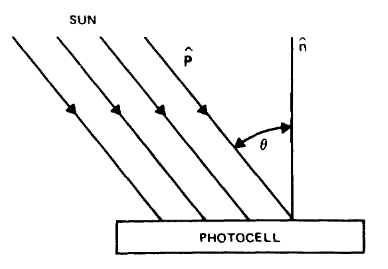
\includegraphics[scale=0.5]{figs/Detector Cossenoildal Sensor Solar.png}
\caption{Sensor Solar de Detecção Cossenoidal}
{Fonte: \cite[p.~156]{wertz2012spacecraft}}
\label{fig:4}
\end{figure}

Para esse modelo, as perdas devido a reflexão de Fresnel, a área efetiva da célula e a reflexão da interface célula-ar dependente do angulo são omitidas.

Para um cubeSat com as células fotovoltaicas encontradas nas seis faces do veículo espacial,  $cos\theta$ pode ser encontrado pela relação do vetor normal do painel $\vec{n}$, com o vetor que aponta para o sol pelo regencial do corpo $\vec{s}^b_{ib}$, sendo ambos unitários.

\begin{equation}
I(\theta)=I(0)cos\theta
\end{equation}
\begin{equation}
I(\theta)=I(0)\vec{n}^T \vec{s}_b
\end{equation}
Utilizando a mesma metodologia para as seis faces tem-se:

\begin{equation}
\mathbf{I}=I(0)\mathbf{N}^T\vec{s}_b
\end{equation}

Sendo $\mathbf{N}$:

\begin{equation}
\mathbf{N}=\begin{bmatrix}
1 & 0 & 0 & -1 & 0 & 0\\ 
0 & 1 & 0 & 0 & -1 & 0\\ 
0 & 0 & 1 & 0 & 0 & -1
\end{bmatrix}\end{equation}

Mas ainda $\vec{s}^b_{ib}$ pode ser encontrado por:

\begin{equation}
\vec{s}_b=C^{B/I}\vec{s}_i\\
\end{equation}
Por fim tem-se:
\begin{equation}
\mathbf{I}=I(0)\mathbf{N}^T C^{B/I}\vec{s}_i
\end{equation}

O sensor magnético ou magnetômetro, fornece a medida do campo magnético terrestre em três eixos. É necessário atenção para o tratamento de ruídos, já que correntes elétricas, campos magnéticos e temperatura, produzidas externas ou internas ao CubeSat interferem nas medições.

Análogo ao caso anterior as medidas do sensor magnético serão dadas utilizando o sistema de referência o de coordenadas do corpo. 

Utilizando um modelo de dipolo inclinado para o campo magnético da terra, é possível escrever seus componentes no SCGI como:

\begin{equation}
m_i^* = \frac{R_T^3H_0}{r^3}\left [ 3\mathbf{d}_i^T\mathbf{\hat{r}}_i\mathbf{\hat{r}}_i-\mathbf{d}_i \right ]
\end{equation}

Onde $\mathbf{d}_i$ é a direção unitária do dipolo no referencial inercial:

\begin{equation}
\mathbf{d}_i=\begin{bmatrix} \sin\theta_m'\cos\alpha_m \\\sin\theta_m'\sin\alpha_m \\ \cos\theta_m'\end{bmatrix}
\end{equation}

Substituindo acima:
\begin{equation}
m_i^*=\frac{R_T^3H_0}{r^3}\begin{bmatrix} 3(\mathbf{d}_i^T\mathbf{\hat{r}}_i)\hat{r}_1 -\sin\theta_m'\cos\alpha_m \\ 3(\mathbf{d}_i^T\mathbf{\hat{r}}_i)\hat{r}_2-\sin\theta_m'\sin\alpha_m \\3(\mathbf{d}_i^T\mathbf{\hat{r}}_i)\hat{r}_3-\cos\theta_m'\end{bmatrix}
\end{equation}

\begin{figure}[htpb]
\centering
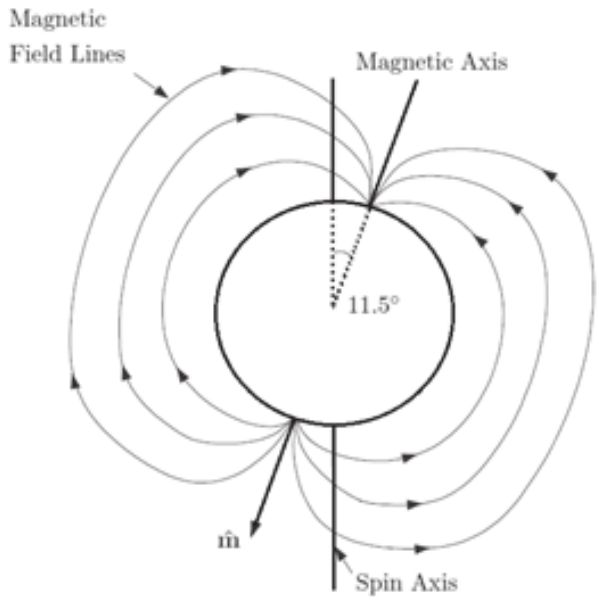
\includegraphics[scale=0.3]{figs/magfield.png}
\caption{Modelo Sensor Magnético}
{Fonte: \cite[p.~13]{mahdi2018attitude}}
\label{fig:5}
\end{figure}

Sendo $r$ o vetor posição do veículo espacial, $R_T$ o raio da Terra, $H_0$ a constante característica do vetor magnético da Terra e $\theta_m'$ co-elevação.

\begin{equation}
\alpha_m = \theta_{go}+\omega_Tt+\phi_m'
\end{equation}

Sendo $\theta_{}go$ a época sideral de greenwich, $\omega_T$ a rotação média da Terra, $t$ o tempo desde a época e $\phi_m'$ a longitude leste do dipolo.

O girômetro do inglês (\textit{rate gyro}) são dispositivos que medem a velocidade angular de um objeto em rotação, esses sensores tem opções mais simples e baratas geralmente adequadas para o controle da taxa de rotação de um cubeSat mas em um sistema com feedback sua saída requer correção frequente para determinação usando outros sensores como solares e magnéticos.

Um girômetro de fibra óptica utiliza o princípio da interferência de luz para medir a rotação ou a orientação angular. Quando a fibra óptica gira, a luz que passa por ela sofre uma mudança de fase, que pode ser medida para determinar a rotação.

As equações de movimento para um girômetro de fibra óptica podem ser expressas da seguinte forma:
 	
\begin{equation}
 		\Delta \phi &= \frac{4 \pi}{\lambda} \cdot L \cdot \Omega
\end{equation}

\begin{equation}
	 		\Omega &= \frac{\Delta \phi \cdot \lambda}{4 \pi \cdot L}
\end{equation}
 	
 	Onde:
 	
\begin{itemize}
 		\item $\Delta \phi$ é a mudança de fase,
 		\item $\lambda$ é o comprimento de onda da luz,
 		\item $L$ é o comprimento da fibra óptica,
 		\item $\Omega$ é a velocidade angular.
\end{itemize}
 

\subsection{Determinação de Atitude: Método TRIAD}\label{sec:3.1.5}

Pelo menos dois vetores são necessários para determinar a atitude. No entanto, é importante notar que, embora sejam necessários três parâmetros independentes para determinar a atitude, cada medição de vetor unitário na verdade fornece apenas dois parâmetros devido à restrição do vetor unitário. Portanto, são necessários três escalares para determinar completamente a atitude. Assim, a exigência é de mais de uma, mas menos de dois medições de vetores. A determinação da atitude é única nesse sentido, pois uma medição não é suficiente, ou seja, o problema é subdeterminado, e duas medições são demais, ou seja, o problema é super-determinado. A principal implicação dessa observação é que todos os algoritmos de determinação de atitude são realmente algoritmos de estimação de atitude.

O algoritmo TRIAD é uma técnica fundamental na determinação da atitude de uma espaçonave. A atitude de uma espaçonave é essencialmente a descrição da matriz de rotação que descreve a orientação do referencial fixo à espaçonave, $B$, em relação a um referencial conhecido, como um referencial inercial, $I$.

Embora essa matriz de cossenos diretores possua nove números, como mostrado anteriormente, apenas três números são necessários para determiná-la completamente. Como cada vetor unitário medido fornece duas informações, são necessárias pelo menos duas medidas diferentes para determinar a atitude o que resulta em um problema super-determinado, pois temos três incógnitas e quatro quantidades conhecidas.

O algoritmo TRIAD parte de dois vetores de medição, como a direção para o sol e a direção do campo magnético terrestre. Denotamos os vetores reais como $\vec{s}$ e $\vec{m}$, respectivamente. As componentes medidas dos vetores, em relação ao referencial do corpo, são denotadas por $\vec{s}_b$ e $\vec{m}_b$, respectivamente. As componentes conhecidas dos vetores no referencial inercial são $\vec{s}_i$ e $\vec{m}_i$.

Idealmente, a matriz de rotação, ou matriz de atitude, $C^{B/I}$, satisfaz $\vec{s}_b=C^{B/I}\vec{s}_i$ e $\vec{m}_b=C^{B/I}\vec{m}_i$. Infelizmente, como o problema é super-determinado, geralmente não é possível encontrar tal $C^{B/I}$. O algoritmo de determinação de atitude determinística mais simples é baseado em descartar uma parte dessa informação no entanto, essa abordagem não se resume simplesmente a descartar uma das componentes de uma das direções medidas. O algoritmo é conhecido como algoritmo TRIAD, porque é baseado na construção de dois triângulos de vetores unitários ortogonais usando as informações vetoriais disponíveis. Os dois triângulos são as componentes do mesmo referencial, denotado por $T$, expresso nos referenciais do corpo e inercial. Este referencial é construído assumindo que um dos pares de vetores corpo/inercial está correto.


\begin{equation}
\begin{bmatrix} \hat{t}_1 \\ \hat{t}_2 \\ \hat{t}_3
\end{bmatrix} = \begin{bmatrix} \hat{s} \\  \hat{s}\times\hat{m} 
\\ \hat{t}_1\times\hat{t}_2
\end{bmatrix}
\end{equation}

\begin{equation}
\begin{bmatrix} \hat{t}_{1b} \\ \hat{t}_{2b} \\ \hat{t}_{3b}
\end{bmatrix} = \begin{bmatrix} \hat{s}_b \\  \hat{s}_b\times\hat{m}_b 
\\ \hat{t}_{1b}\times\hat{t}_{2b}
\end{bmatrix}
\end{equation}

\begin{equation}
\begin{bmatrix} \hat{t}_{1i} \\ \hat{t}_{2i} \\ \hat{t}_{3i}
\end{bmatrix} = \begin{bmatrix} \hat{s}_i \\  \hat{s}_i\times\hat{m}_i
\\ \hat{t}_{1i}\times\hat{t}_{2i}
\end{bmatrix}
\end{equation}

\begin{equation}
C^{B/I} = C^{B/T}C^{B/I}=\left [\hat{t}_{1b} \hat{t}_{2b} \hat{t}_{3b}  \right ]
\begin{bmatrix} \hat{t}_{1i}\\\hat{t}_{2i}\\\hat{t}_{3i}
\end{bmatrix}
\end{equation}

\subsection{Controle de Atitude: Técnica de Controle PID}\label{sec:3.1.6}

Para o controle da atitude do CubeSat por rodas de reação se usa um controlador automático estes comparam o valor de saída, medido por um sensor, com o valor de entrada, de referência, desejado. A comparação desses dois valores determina um desvio chamado de erro, e esse sinal de erro é tratado pelo controlador que gera por fim um sinal de controle para os atuadores que agiram sobre o sistema na busca de diminuir esse desvio. A técnica aqui demostrada está presente em \cite[p.~21]{ogata2011engenharia}.

O controle proporcional-integral-derivativo ou PID, é um controle automático que combina ações de natureza proporcional, integral e derivativa no tratamento do sinal de erro. Essa ação combinada oferece as vantagens induviais de cada um desses tipo de controle. 
A utilização de rodas de reação quando o controle é feito por velocidade, no presente caso aplica-se um controlador PID ao sinal de corrente. Dessa forma a equação do sinal de controle é dada por:

\begin{equation}
u(t)=K_p\left(e(t)+\frac{1}{T_i}\int_{0}^{t}e(t)dt+T_d\frac{\mathrm{d}e(t) }{\mathrm{d} t}\right )
\end{equation}

Onde $e(t)$ é o erro entre a velocidade angular de referência e a observada, $K_p$ é o ganho proporcional, $T_i$ é o tempo integrativo e $T_d$ é o tempo derivativo.

Para o caso que o modelo matemático da planta a ser considerada possa ser obtido, então é possível aplicar técnicas de projeto para auxiliar na determinação de parâmetros do controlador para atender as especificações do regime transitório e do regime permanente do sistema de malha fechada. Contudo se a planta for muito complexa é possível que a abordagem analítica seja não praticável, assim tem-se que recorrer para uma abordagem experimental de sintonia do controlador PID.

O método de sintonia  de Ziegler e Nichols, \cite[p.~524]{ogata2011engenharia}, sugere ajustar os parâmetros $Kp$, $T_i$ e $T_d$ a partir da resposta experimental ao aumentar o valor de $K_p$ até resultar em uma estabilidade marginal, quando só a ação proporcional é considerada. Ou seja, definindo $T_i=\infty$ e $T_d=0$, aumenta-se o valor de $K_p$ de 0 até o valor crítico $K_{cr}$no qual a saída oscila de forma sustentada pela primeira vez, o período de oscilação encontrado é $P_{cr}$. Caso para qualquer valor de $K_p$ não se encontre uma resposta oscilatória sustentada do sistema então o método não se aplica.

Para os valores de $P_{cr}$ e $K_{cr}$encontrados Ziegle e Nichols sugere escolher os parâmetros $Kp$, $T_i$ e $T_d$ de acordo com a  tabela~\ref{tab:1} a seguir:

\begin{table}[htpb]
\centering
\caption{Regra de sintonia de Ziegler-Nichols baseada no ganho crítico $K_{cr}$ e no período crítico $P_{cr}$.}\label{tab:1}
\begin{tabular}{|c|c|c|c|}
\hline
\small{Tipo de controlador} & \small{$K_p$} & \small{$T_i$} & \small{$T_d$} \\ \hline
P&$0,5K_{cr}$&$\infty$&$0$\\\hline
PI& $0,45K_{cr}$&$\frac{1}{1,2}P_{cr}$&$0$\\\hline
PID	& $0,6K_{cr}$&$0,5P_{cr}$&$0,125P_{cr}$\\\hline
\end{tabular}
\end{table}


\subsection{Rodas de Reação em 3 Eixos}\label{sec:3.1.6.1}


As rodas de reação (RDR) são dispositivos atuadores utilizados para o controle de atitude de veículos espaciais, possuindo, como a base de seu funcionamento, a transferência de momento angular. Podendo ser arranjadas em conjuntos de três unidades para controlar a rotação nos três eixos, de quatro unidades para além dos controles dos três eixos oferecer redundância ao sistema, ou avulso.

Por permitirem a correção de atitude com precisão, estes dispositivos têm operação mais complexa e são mais custosos. Apenas em missões nas quais os requisitos do apontamento são mais sensíveis se utiliza esse tipo de atuador, sendo assim menos comuns em CubeSats.

Contudo, com o aumento de missões mais rebuscadas, estas que se encontram distante do campo magnético da Terra, faz-se mais necessário esses dispositivos, deste modo, se tornando comuns e até comercializados, que é o caso da SatBus 4RW0, um conjunto de 4 rodas de reação desenvolvidas pela NanoAvionics para seus CubeSats (M3P ao M16P),  também podendo ser encomendadas, e a CubeWhell encontrada na CubeSat Shop e a Blue Canyon com sistemas completamente integrados de ADCS com rodas de reação acopladas,  Figura~\ref{fig:10}.


Uma roda de reação é uma massa rotativa motorizada que fornece torque para manobra e é usada para o apontamento de satélites. Podendo rotacionar tanto no sentido horário quanto no anti-horário, assim como acelerar ou desacelerar, criando torques e manobrando o satélite.

Esse dispositivo necessita de uma forma de dessaturar ao longo do tempo, assim um sistema adicional podendo ser torqueadores magnéticos ou propulsores cumprem essa função descarregando o momento angular.

Mais precisamente uma roda de reação consistem em cilindros de metal encaixadas em um motor sem escova achatado, é indispensável que esse motor tenha uma boa relação potência consumo e que funcione dentro da faixa de potência oferecida por esse sistema do satélite. Estas rodas de reação permitem um alto grau de acurácia e são essenciais em missões as quais um controle mais fino e robusto é necessário.

Variando entre 0,4 a 40 $\frac{kg\;m^2}{s}$, podendo ser uma roda pequena e rápida ou uma roda grande e lenta. Esses dispositivos se baseiam no principio da conservação de momento, \textit{i.e.}, $\vec{H}=J^b_{RDR}\;\vec{\omega}_{RDR}$. Onde $\vec{\omega}_{RDR}$ é o vetor das velocidades angulares e $J^b_{RDR}$ a matriz de inércia da roda-de-reação. O modelo utilizado para a caracterização física-matemática da roda de reação foi adaptado de \cite[p.~270-271]{wertz2012spacecraft}.

O torque da roda é oferecido por um motor de indução elétrica de corrente contínua, alimentado por pulsos quadrados provenientes da bateria controlados pelo computador de bordo ao nível do ciclo de trabalho, que está relacionado com a velocidade de rotação da roda.

O Ciclo de trabalho $X_{ct}$ varia entre +1 e -1 a partir do sinal de controle, $V$, mostrado na Figura~\ref{fig:14}.

\begin{figure}[htpb]
\centering
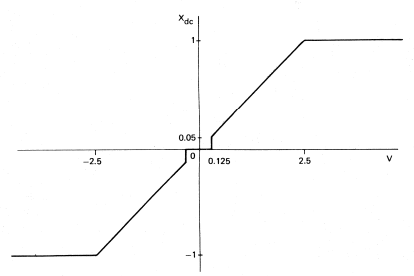
\includegraphics[scale=1]{figs/CicloTrabalho.png}
\caption{Ciclo de Trabalho $X_{CT}$}
{Fonte: \cite[p.~271]{wertz2012spacecraft}}
\label{fig:6}
\end{figure}

O torque líquido é encontrado por:

\begin{equation}N=X_{ct}N_{em}-N_{fricção}\end{equation}

Onde $N_{em}$ é o torque eletromagnético produzido por indução, e $N_{fricção}$ contabiliza o atrito viscoso e de Coumlomb, descrito por:

\begin{equation}N_{fricção}=N_c\left (\frac{s}{|s|}\right )+f\;s\end{equation}

Onde $N_c$ é o coeficiente de fricção de Coulomb, $f$ é o coeficiente de fricção viscosa e $s$ a velocidade de rotação da roda.

Para encontrar o torque eletromagnético, $N_{em}$, pode-se se utilizar a seguinte aproximação:

\begin{equation} N_{em} = \frac{2N_0\alpha\;r}{(\alpha^2+r^2)}\end{equation}

Sendo, $N_0$ a magnitude máxima de $N_{em}$, $\alpha$ é o valor de $r$ onde se encontra $N_0$ e $r$ é encontrado pela seguinte relação:

\begin{equation}r=1-\frac{s}{s_{max}}\;\text{para}\;X_{ct}>0 \end{equation}\begin{equation} r=1+\frac{s}{s_{max}}\;\text{para}\;X_{ct}<0\end{equation}

Atente-se que $s_{max}$ é conhecida pela velocidade de sincronização da roda-de-reação. O torque eletromagnético em relação a velocidade da roda é mostrado na Figura~\ref{fig:15}.

\begin{figure}[htpb]
\centering
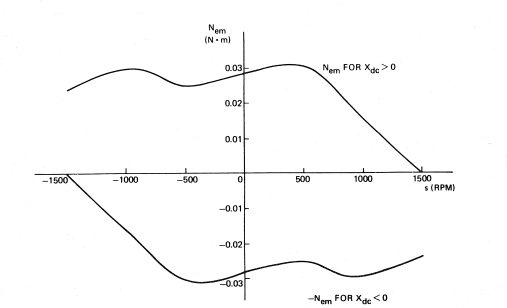
\includegraphics[scale=1]{figs/torqueEletromagnetico.png}
\caption{Torque Eletromagnético $N_{em}$ em relação a velocidade de rotação da roda-de-reação $s$}
{Fonte: \cite[p.~271]{wertz2012spacecraft}}
\label{fig:15}
\end{figure}

\subsection{Modelagem das Rodas-De-Reação}\label{sec:3.1.6.2}

A equação para uma roda-de-reação, controlada por uma corrente contínua $i(t)$ ao invés de uma tensão de controle, e, utilizando os modelos de zona ociosa,  torque eletromagnético, fricção viscosa e o coeficiente do torque de Coulomb descritos acima, é dada por:

\begin{equation}
T_{aplicado}=J_{axial}\frac{d\omega_{rdr}}{dt}=Xct(i(t))\frac{2N_0\alpha\left (1-\frac{\omega_{rdr}}{\omega_{rdr\;max}} \right )}{\alpha^2\left (1-\frac{\omega_{rdr}}{\omega_{rdr\;max}} \right )^2}-\left (sign(Xct(i(t)))N_c+f\omega_{rdr}\right )
\end{equation}
Como as três rodas-de-reação são idênticas, pode-se modela-las como cilindros de metal com massa uniformemente distribuída, onde $m_{rdr}$ é a massa e $\{\rho_{rdr}\}$ o raio:

\begin{equation}{J_{axial}}=\frac{m}{2}\rho^2_{rdr}\end{equation}Contabilizando somente as componentes axiais das rodas de reação e alinhando cada com eixos principais de inercia da matriz de inércia coincidentes ao sistema de referencia fixa no corpo, tem-se que   $J^b_{rdr}$:

\begin{equation}J^b_{rdr} =\begin{bmatrix}
{J_{axial}}_1&0&0 \\0 &{J_{axial}}_2&0 \\ 0&0&{J_{axial}}_3
\end{bmatrix}\end{equation}E aplicando a modelagem para cada eixo, tem-se que o vetor de torques aplicado fica:
\begin{equation}
\vec{T}_{aplicado}=J^b_{rdr}\frac{d\vec{\omega^b_{rdr}}}{dt}
\end{equation}


\subsection{Linearização do Modelo das Rodas de Reação}\label{sec:3.1.6.3}




